The   LT3741's   \emph{Enable}   input   is   enabled   and   disabled   by  the
microcontroller's  $BUCK\_EN$ signal on one hand, on the other hand it is can be
forcibly  disabled  in  hardware  when  the  \SI{28}{\volt}  rail   drops  below
\SI{25}{\volt}. This  allows  for  a  controlled and predictable behavior of the
LT3741 during power-on  and power-off. The corresponding circuit can be found in
figure \ref{fig:circuit:uvlo}.

\begin{figure}[th!]
    \center
    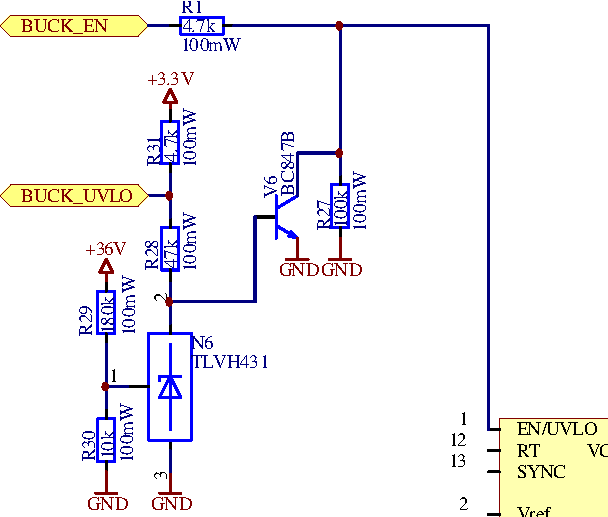
\includegraphics[width=.6\textwidth]{images/circuit/uvlo.pdf}
    \caption{Under-Voltage Lock-Out (UVLO) allows for controlled power-on and power-off of the controller}
    \label{fig:circuit:uvlo}
\end{figure}

In case of under-voltage, $N_6$ switches  on  and the transistor $V_6$ starts to
conduct,  thus  pulling  the  \emph{Enable}   input   to   \emph{Low}.   Voltage
$BUCK\_UVLO$ triggers an interrupt in the microcontroller.

